\chapter{System Description}\label{chap:systemDescription}
The system is composed by a camera that captures the table that contains the bricks and a robot arm that is charge of picking and placing the brick to build the desired figures. The setup can be seen in \autoref{fig:setup}.

%\begin{figure}
%    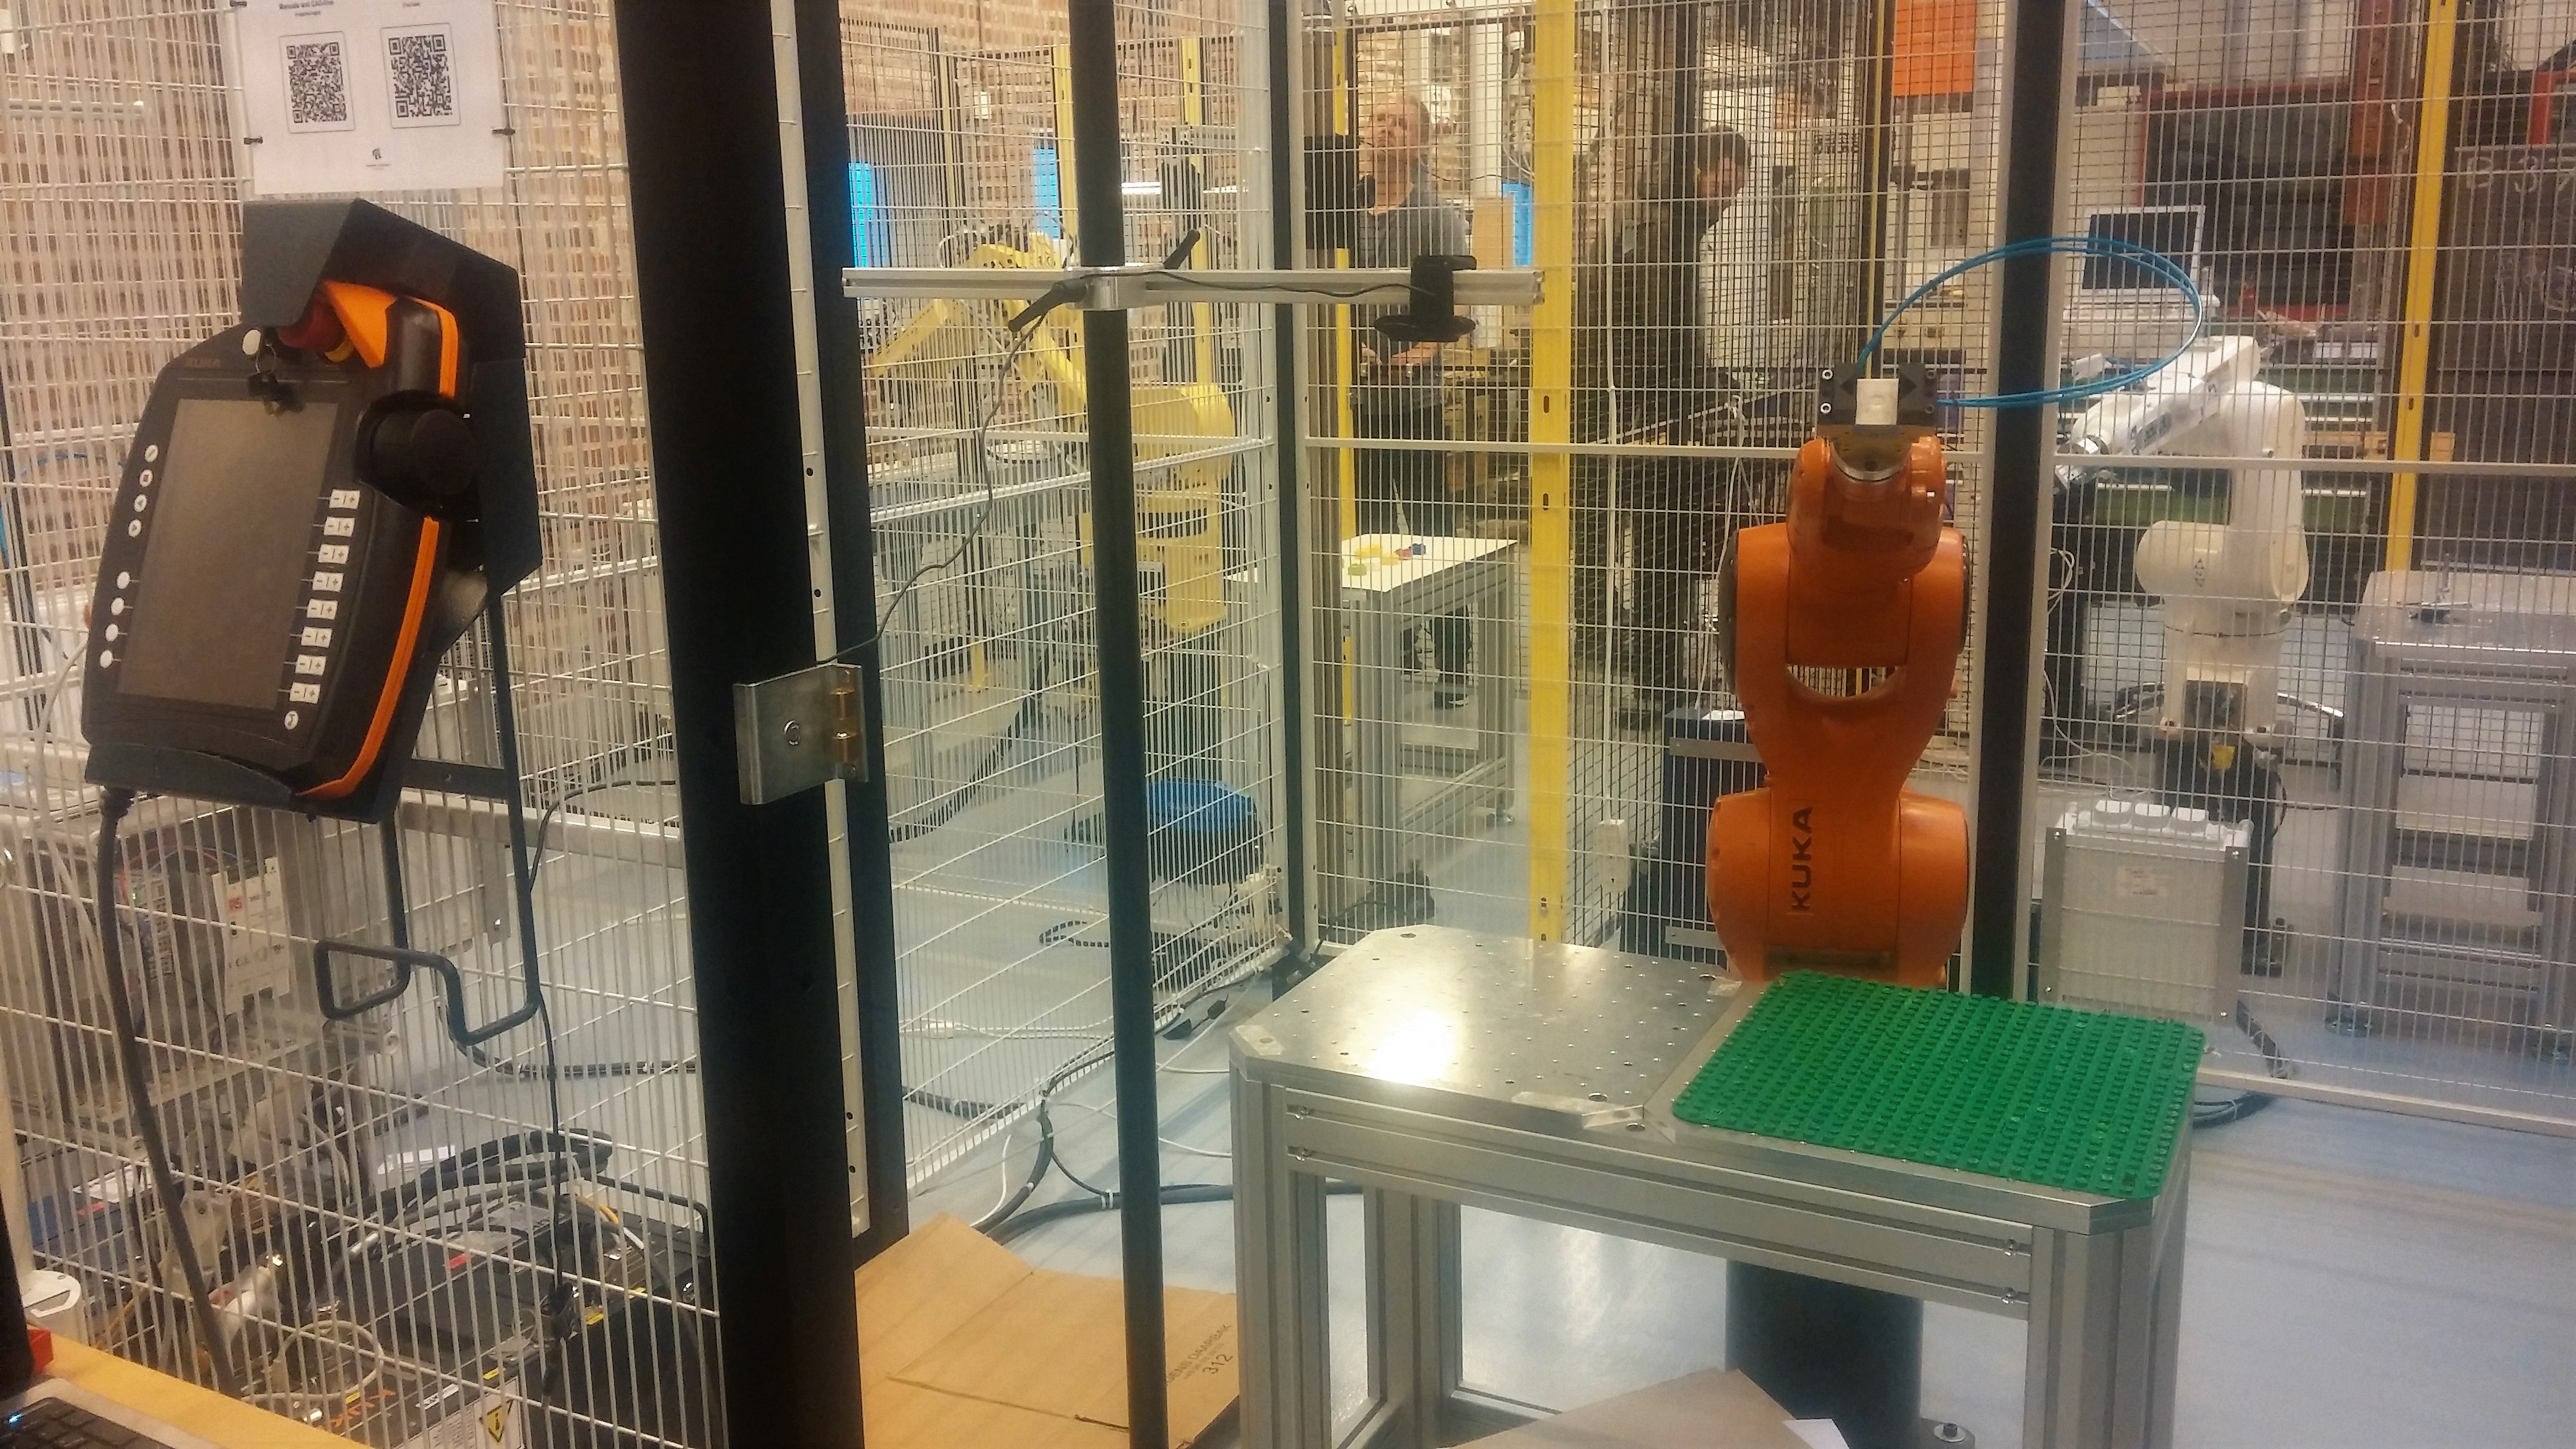
\includegraphics[width=0.4\textwidth]{figures/setup}
%    \caption{Image of the setup, where the robot cell can be seen. It contains the robot arm, the security fence, the camera and the table that is the base workspace of the system. }
%    \label{fig:setup}
%\end{figure}

In this chapter more details about the robot arm and the camera are described, including the definition of the coordinate system used to send references to the robot and the camera calibration. 

\section{Robot Arm}
The robot arm is a KUKA KR6 R700.
\begin{figure}[H]
    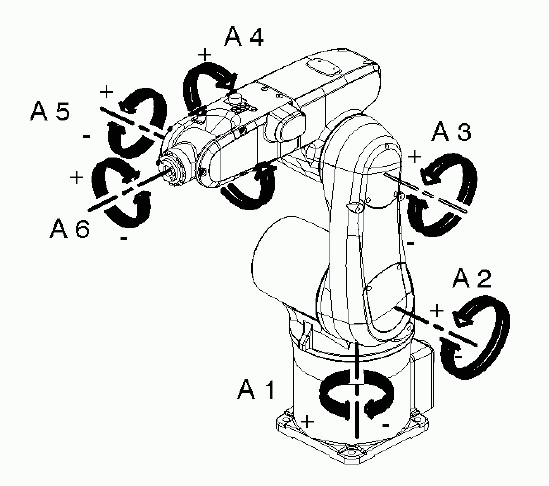
\includegraphics[width=0.4\textwidth]{figures/kuka_axes.jpg}
    \caption{.\cite{kuka} }
    \label{fig:kuka_axes}
\end{figure}


Gripper description

\section{Camera}
\begin{figure}[H]
    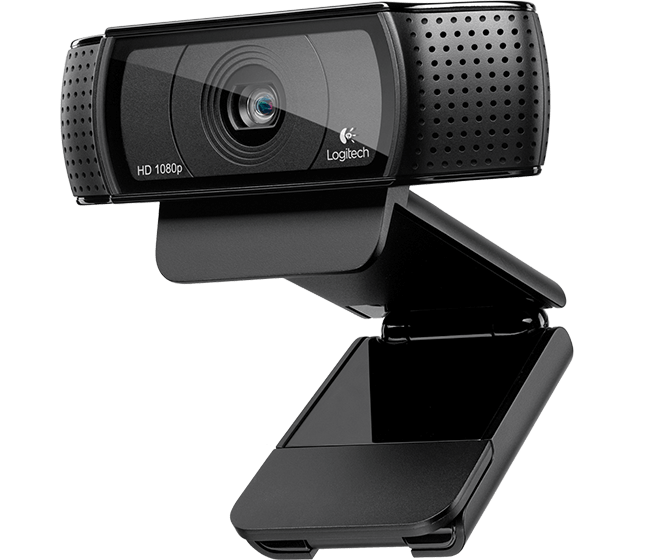
\includegraphics[width=0.2\textwidth]{figures/camera.png}
    \caption{.\cite{camera} }
    \label{fig:camera}
\end{figure}

Calibration
Projection matrix

